\documentclass{beamer}
\definecolor{azulPoP}{rgb}{0.243,0.466,0.701}
\mode<presentation> {
%\usetheme{Warsaw}
\setbeamercolor{frametitle}{fg=white,bg=azulPoP}
\setbeamercolor{subsection in head/foot}{fg=white,bg=black}
\setbeamercolor{block title}{bg=azulPoP,fg=white}
\setbeamercolor{title}{bg=azulPoP,fg=white}
}

\usepackage{graphicx} % Allows including images
\usepackage{booktabs} % Allows the use of \toprule, \midrule and \bottomrule in tables
\usepackage[utf8x]{inputenc}
\usepackage{minted}
\usepackage[portuges]{babel}
%----------------------------------------------------------------------------------------
%	TITLE PAGE
%----------------------------------------------------------------------------------------
\setbeamerfont{footnote}{size=\tiny}
\title[Introdução à Orientação a Objetos I]{Introdução à Orientação a Objetos I} % The short title appears at the bottom of every slide, the full title is only on the title page

\author{Rafael Silva Guimarães} % Your name
\institute[IFES] 
{
Instituto Federal do Espírito Santo \\ % Your institution for the title page
\medskip
\textit{rafaelg@ifes.edu.br} \\ % Your email address
\textit{http://rafaelguimaraes.net} \\
\textit{https://github.com/rafaelsilvag/ifesJava/}
}
\date{\today} % Date, can be changed to a custom date
\logo{
\includegraphics[scale=0.2]{imagens/ifes.png}}

\begin{document}

\setbeamertemplate{footline}
{%
\leavevmode%
\hbox{%

%\begin{beamercolorbox}[wd=.20\paperwidth,ht=1.0ex,dp=1.125ex,left]{author
%in head/foot}%
%\usebeamerfont{title in head/foot}\insertshortauthor\hspace{.3cm}
%\end{beamercolorbox}%

\begin{beamercolorbox}[wd=.45\paperwidth,ht=0.8ex,dp=1.125ex,left]{title
in head/foot}%
\usebeamerfont{author in head/foot}\hspace{.3cm}\insertshorttitle

\end{beamercolorbox}%

\begin{beamercolorbox}[wd=.1\paperwidth,ht=0.8ex,dp=1.125ex,center]{title
in head/foot}%
\usebeamerfont{author in head/foot}\insertframenumber/\inserttotalframenumber
\end{beamercolorbox}%
}%
\vskip0pt%
}

\begin{frame}
\titlepage % Print the title page as the first slide
\end{frame}

\begin{frame}
\frametitle{Glossário} % Table of contents slide, comment this block out to remove it
\tableofcontents % Throughout your presentation, if you choose to use \section{} and \subsection{} commands, these will automatically be printed on this slide as an overview of your presentation
\end{frame}

%----------------------------------------------------------------------------------------
%	PRESENTATION SLIDES
%----------------------------------------------------------------------------------------

%------------------------------------------------
\section{Parte 1} % Sections can be created in order to organize your presentation into discrete blocks, all sections and subsections are automatically printed in the table of contents as an overview of the talk
%------------------------------------------------

\subsection{Histórico} % A subsection can be created just before a set of slides with a common theme to further break down your presentation into chunks

\begin{frame}
\frametitle{Histórico}
\begin{itemize}
\item Em 1995, a Sun Microsystem\textregistered\ anunciou o Java; não era apenas mais uma linguagem de programação, mas uma plataforma de desenvolvimento.  
\item Atualmente o Java está na versão 8 com algumas mudanças interessantes a caminho na versão 9, obviamente, de domínio da Oracle. Em 2007 a Sun Microsystem abriu o projeto Java para a comunidade através do projeto OpenJDK. Apesar disso, atualmente as VMs Oracle\textregistered, através da aquisição da Sun, e OpenJDK, não conseguem ter 100\% de compatibilidade.
\\
	\begin{figure}[h!]
		\centering
		
\includegraphics[scale=0.1]{imagens/oracle}
		
\includegraphics[scale=0.1]{imagens/sun}
	\end{figure}
\end{itemize}
\end{frame}

\subsection{A Linguagem Java}

\begin{frame}
	\frametitle{A Linguagem Java}
	\begin{itemize}
		\item Características da Linguagem Java:
		\begin{itemize}
			\item[-] \textbf{Orientação a objetos:} é uma prática de programação já sólida no mercado e na maioria das linguagens de hoje.
			\item[-] \textbf{Portabilidade:} Java é uma linguagem multiplataforma, ou seja, uma mesma aplicação pode ser executada em diferentes tipos de plataforma sem a necessidade de adaptação do código. Vamos para um exemplo prático!
			\item[-] \textbf{Multithreading:} é o meio pelo qual se consegue fazer com que mais de um evento aconteça simultaneamente em um programa.
		\end{itemize}
	\end{itemize}
\end{frame}
\begin{frame}
	\frametitle{A Linguagem Java}
	\begin{itemize}
		\item Características da Linguagem Java:
		\begin{itemize}
			\item[-] \textbf{Suporte à comunicação:} Java detém de um grande conjunto de classes(bibliotecas) com funcionalidades específicas, ou seja, um alto nível de manipulação já estão encapsuladas em classes prontas, acelerando o desenvolvimento. Neste contexto, temos classes que já suportam a manipulação de tecnologias de comunicação, tais como: TCP/IP, HTTP, FTP, etc.
			\item[-] \textbf{Acesso remoto a um banco de dados:} No Java utiliza-se classes prontas, criadas pela Sun Microsystem, para realizar a manipulação de SGBD.
		\end{itemize}
	\end{itemize}
\end{frame}

\begin{frame}
	\frametitle{A Plataforma Java}
	\begin{figure}[h!]
		\centering
		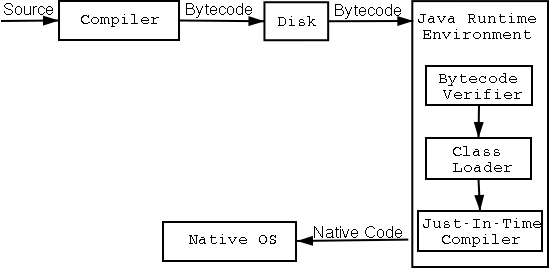
\includegraphics[scale=0.55]{imagens/java-compilation}
	\end{figure}
\end{frame}

\begin{frame}
	\frametitle{A Plataforma Java}
	\begin{figure}[h!]
		\centering
		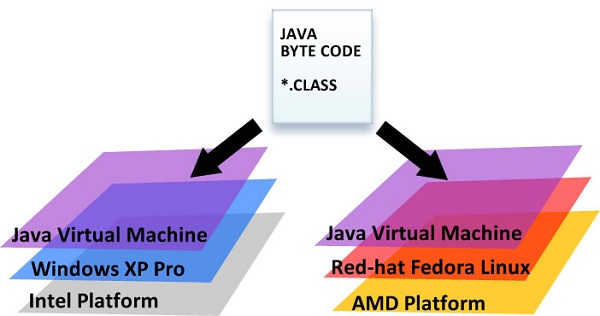
\includegraphics[scale=0.45]{imagens/java-vm}
	\end{figure}
\end{frame}

\subsection{Ambiente de Desenvolvimento}

\begin{frame}
	\frametitle{Ambiente de Desenvolvimento}
	\begin{itemize}
		\item Existem diversas ferramentas para realizarmos o desenvolvimento de programas Java. Na maioria dos casos, estas ferramentas são multiplataformas e podem ser executadas em diversos sistemas operacionais. As principais são:
		\begin{itemize}
			\item[-] Eclipse
			\item[-] NetBeans
		\end{itemize}
		\item Além disso, precisamos do Kit de Desenvolvimento da Sun/Oracle, para conseguirmos gerar o código intermediário de um determinado programa. Segue as informações de cada plataforma:
		\begin{itemize}
			\item[-] JRE(Java Runtime Environment): Responsável por executar o programa através de seu código intermediário(Bytecode).
			\item[-] JDK(Java Development Kit): Responsável por gerar o código intermediário a partir de um determinado programa escrito na linguagem Java.
		\end{itemize} 
	\end{itemize}
\end{frame}

\subsection{Primeiro Contato}

\begin{frame}
	\frametitle{Primeiro Contato}
	\begin{example}[Primeiro Contato - PrimeiroContato01.java]
		\inputminted{java}{codigos/PrimeiroContato01.java}
	\end{example}
\end{frame}

\begin{frame}
	\frametitle{Primeiro Contato}
	\begin{itemize}
		\item \textbf{Public}: É um qualificador do método ou da classe que indica que ele é acessível externamente a essa classe por outra classe. 
		\item \textbf{Static}: Qualificador que indica que o método deve ser compartilhado por todos os objetos que são criados a partir dessa classe.
		\item \textbf{Void}: É o valor de retorno do método. Funcionalidade idêntica da utilizada na linguagem C. Aliás, verão que a sintaxe de muitos comandos são idênticas da linguagem C, principal causa de uma fácil transição entre estas linguagens.
		\item \textbf{Main}: Este é o nome do método que indica ao compilador o início do programa.
	\end{itemize}
\end{frame}

\section{Parte 2}

\subsection{Tipos de Dados}
% Declaração de variáveis
\begin{frame}
	\frametitle{Tipos de Dados}
	\begin{itemize}
		\item A linguagem de programação Java não tem tipagem dinâmica, necessitanto sempre mencionar o tipo de dado que será utilizado naquela determinada variável.
		\item Neste caso, a linguagem fornece alguns tipos primitivos da linguagem, como mostra na tabela abaixo:
	\end{itemize}
	\begin{table}
		\begin{tabular}{cl l}
			\toprule
			\textbf{Tipo} & \textbf{Qtd de Bits} \\
			\midrule
			char & 16 \\
			byte &  8 \\
			int & 32 \\
			short & 16 \\
			long & 64 \\
			float & 32 \\
			double & 64 \\
			boolean & 8 ( true ou false )\\
			\bottomrule
		\end{tabular}
		%\caption{Tipos Primitivos em Java}
	\end{table}
\end{frame}

\begin{frame}
	\frametitle{Tipos de Dados}
	\begin{example}[TiposDados01.java]
		\inputminted{java}{codigos/TiposDados01.java}
	\end{example}
\end{frame}

% Exemplos de declaracao
\begin{frame}
	\frametitle{Nomes das variáveis}
	\begin{itemize}
		\item Os nomes de variáveis devem começar com letra, caracteres de sublinhado(\_) ou cifrão (\$). \textbf{Não é permitido iniciar o nome de uma variável com número}.
		\item Por convenção, a linguagem Java utiliza o seguinte padrão para nomear as variáveis:
		\begin{itemize}
			\item[-] Quando o nome da variável for composto apenas por um caractere ou palavra, os caracteres devem ser minúsculos.
			\item[-] Quando o nome da variável tiver mais de uma palavra, a primeira letra, da segunda palavra em diante, devem ser maiúsculas. Todos os outros caracteres devem ser minúsculos.
		\end{itemize}
		\item Exemplos: a, a1, x, tempo, nome, valorVenda, codigoFornecedor.
	\end{itemize}
\end{frame}	
% Constantes
\begin{frame}
	\frametitle{Constantes em Java}
	\begin{itemize}
		\item Não existe constantes em Java, o que existe é um tipo de variável com comportamento semelhante a uma constante de outras linguagens. É na verdade um tipo de variável que não pode ter o seu conteúdo alterado depois de ter sido inicializada. Em Java, essa variável é chamada de final, exemplo:
	\end{itemize}
	\inputminted{java}{codigos/TiposDados02.java}
\end{frame}

\subsection{Operadores}
% Operadores
\begin{frame}
	\frametitle{Operadores Aritméticos}
	\begin{table}
		\begin{tabular}{cl l}
			\toprule
			\textbf{Função} & \textbf{Sinal} & \textbf{Exemplo} \\
			\midrule
			Adição & + & x + y \\
			Subtração & - & x - y \\
			Multiplicação & * & x * y \\
			Divisão & / & x / y \\
			Resto da Divisão & \% & x \% y \\
			Sinal Negativo & - & -x \\
			Sinal Positivo & + & +x \\
			Incremento Unitário & ++ & ++x ou x++ \\
			Decremento Unitário & - - & - -x ou x- - \\
			\bottomrule
		\end{tabular}
		\caption{Operadores Aritméticos}
	\end{table}
\end{frame}
\begin{frame}
	\frametitle{Operadores Relacionais}
	\begin{table}
		\begin{tabular}{cl l}
			\toprule
			\textbf{Função} & \textbf{Caractere(s) utilizados(s)} & \textbf{Exemplo} \\
			\midrule
			Igual & == & x == y \\
			Diferente & != & x != y \\
			Maior que & \textgreater & x \textgreater\ y \\
			Maior ou igual a & \textgreater= & x \textgreater= y \\
			Menor que & \textless & x \textless\ y \\
			Menor ou igual a & \textless= & x \textless= y \\
			\bottomrule
		\end{tabular}
		\caption{Operadores Relacionais}
	\end{table}
\end{frame}
\begin{frame}
	\frametitle{Operadores Lógicos}
	\begin{table}
		\begin{tabular}{cl l}
			\toprule
			\textbf{Operador} & \textbf{Ação} \\
			\midrule
			\&\& & AND (E) \\
			\textbar \textbar & OR (OU) \\
			! & NOT (NÃO) \\
			\bottomrule
		\end{tabular}
		\caption{Operadores Lógicos}
	\end{table}
\end{frame}

%%%% Tipos Primitivos - Imagem
%\begin{frame}
%\frametitle{Tipos Primitivos}
%	\begin{figure}[h!]
%		\centering
%		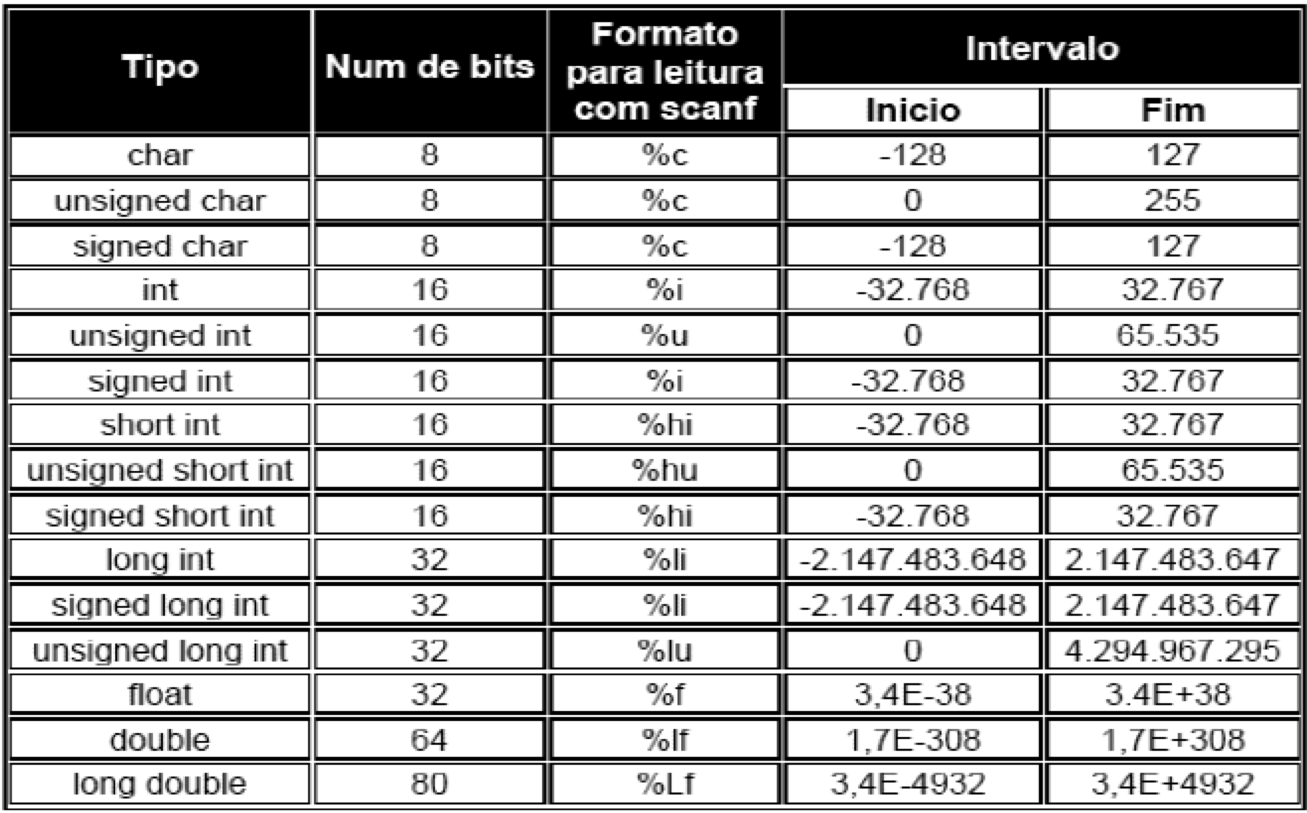
\includegraphics[scale=0.47]{imagens/tiposvariaveis}
%	\end{figure}
%\end{frame}
%
%%%% Declaração de variáveis
%\begin{frame}
%	\frametitle{Declaração de Variáveis}
%	\begin{itemize}
%		\item As variáveis no C devem ser declaradas antes de serem usadas. A forma geral da declaração de variáveis é:
%	\end{itemize}
%	\begin{center}
%		\textbf{	tipo\_da\_variável   	lista\_de\_variáveis; }
%	\end{center}	
%	\begin{example}[Declaração de Variáveis]
%		\inputminted{c}{codigos/variaveis.c}
%	\end{example}	
%\end{frame}
%
%%%% Definição do Início e do Fim de um Algoritmo
%\begin{frame}
%	\frametitle{Definição do Início e do Fim de um Algoritmo}
%	\begin{itemize}
%		\item No Visualg o início e o fim do algoritmo eram definidos pelas palavras: inicio e fimalgoritmo
%		\item Em C um algoritmo é definido da seguinte forma:
%	\end{itemize}
%	\begin{example}[Início e Fim do Algoritmo]
%		\inputminted{c}{codigos/iniciofim.c}
%	\end{example}	
%\end{frame}
%
%\subsection{Entrada e Saída}
%%% Introdução a entradas e saídas
%\begin{frame}
%	\frametitle{ Introdução a Entradas e Saídas}
%	\begin{itemize}
%		\item No Visualg quando desejávamos escrever algo na tela utilizávamos o comando escreva
%		\item Em C, o comando equivalente é o \textbf{printf} que pode ser definido da seguinte forma:
%	\end{itemize}
%	\begin{example}[Saída]
%		\inputminted{c}{codigos/saida.c}
%	\end{example}
%\end{frame}
%
%%% Introdução a entradas e saídas
%\begin{frame}
%	\frametitle{ Introdução a Entradas e Saídas}
%	\begin{itemize}
%		\item Exemplo de uso do \textbf{printf}:
%		\begin{example}[Uso do \textbf{printf}]
%			\inputminted{c}{codigos/saidaexemplo.c}
%		\end{example}
%		\begin{itemize}
%			\item[-] Onde número é uma variável do tipo inteiro.
%			\item[-] O \textbf{\textbackslash{n}} é o comando utilizado para que após a escrita da mensagem seja feito o 'pular de linha'.
%		\end{itemize}
%	\end{itemize}
%\end{frame}
%
%%% Introdução a entradas e saídas
%\begin{frame}
%	\frametitle{ Introdução a Entradas e Saídas}
%	\begin{itemize}
%		\item No Visualg quando desejávamos ler algo na tela utilizávamos o comando leia
%		\item Em C o comando equivalente é o \textbf{scanf} que pode ser definido da seguinte forma:
%		\begin{example}[Uso do \textbf{scanf}]
%			\inputminted{c}{codigos/entrada.c}
%		\end{example}
%	\end{itemize}
%\end{frame}
%
%%% Introdução a entradas e saídas
%\begin{frame}
%	\frametitle{ Introdução a Entradas e Saídas}
%	\begin{itemize}
%		\item Exemplo de uso do \textbf{scanf}:
%		\begin{example}[Uso do \textbf{scanf}]
%			\inputminted{c}{codigos/entrada.c}
%		\end{example}
%		\begin{itemize}
%			\item[-] Onde meses é uma variável do tipo inteiro.
%		\end{itemize}
%	\end{itemize}
%\end{frame}
%
%\subsection{Operadores}
%%%Operadores aritméticos
%\begin{frame}
%	\frametitle{Operadores Aritméticos}
%	\begin{table}
%		\begin{tabular}{cl l}
%			\toprule
%			\textbf{Operador} & \textbf{Ação} \\
%			\midrule
%			+ & Soma (Inteira e ponto flutuante)  \\
%			 - & Subtração ou troca de sinal(inteira ou ponto flutuante) \\
%			 * & Multiplicação (inteira ou ponto flutuante) \\
%			 / & Divisão (inteira ou ponto flutuante) \\
%			 \% & Resto da Divisão (de inteiros) \\
%			++ & Incremento (inteira ou ponto flutuante) \\
%			- - & Decremento (inteira ou ponto flutuante) \\			 
%			\bottomrule
%		\end{tabular}
%		\caption{Operadores Aritméticos}
%	\end{table}
%\end{frame}
%
%\begin{frame}
%	\frametitle{Operadores Relacionais}
%	\begin{table}
%		\begin{tabular}{cl l}
%			\toprule
%			\textbf{Operador} & \textbf{Ação} \\
%			\midrule
%			\textgreater & Maior do que \\
%			\textgreater = & Maior ou igual a \\
%			\textless & Menor do que \\
%			\textless = & Menor ou igual a \\
%			== & Igual a \\
%			!= & Diferente de \\	 
%			\bottomrule
%		\end{tabular}
%		\caption{Operadores Relacionais}
%	\end{table}
%\end{frame}
%
%\begin{frame}
%	\frametitle{Operadores Lógicos}
%	\begin{table}
%		\begin{tabular}{cl l}
%			\toprule
%			\textbf{Operador} & \textbf{Ação} \\
%			\midrule
%			\&\& & AND (E) \\
%			\textbar \textbar & OR (OU) \\
%			! & NOT (NÃO) \\
%			\bottomrule
%		\end{tabular}
%		\caption{Operadores Lógicos}
%	\end{table}
%\end{frame}
%
%\begin{frame}
%	\frametitle{Operador de Atribuição}
%	\begin{itemize}
%		\item A atribuição de um valor a uma variável é algo bem simples. Basta utilizar o símbolo "=".
%		
%		\inputminted{c}{codigos/atribuicao.c}
%	\end{itemize}
%\end{frame}

%------------------------------------------------
\subsection{Referências}

\begin{frame}
	\frametitle{Referências}
	\footnotesize{
		\begin{thebibliography}{99} % Beamer does not support BibTeX so references must be inserted manually as below
			\bibitem[Cornell, G. ; Horstmann, S. C., 2003]{p1} Cornell, G. ; Horstmann, S. C. 
			\newblock Core Java 2: Fundamentos (vol.1.)
			\newblock \emph{Pearson Makron Books} São Paulo
		\end{thebibliography}
		\begin{thebibliography}{99} % Beamer does not support BibTeX so references must be inserted manually as below
			\bibitem[Cornell, G. ; Horstmann, S. C., 2003]{p2} Cornell, G. ; Horstmann, S. C. 
			\newblock Core Java 2: Recursos Avançados (vol.2.)
			\newblock \emph{Pearson Makron Books} São Paulo
		\end{thebibliography}
		\begin{thebibliography}{99} % Beamer does not support BibTeX so references must be inserted manually as below
			\bibitem[Sebesta, R.W., 2003]{p3} Sebesta, R.W.
			\newblock Conceitos de Linguagens de Programação
			\newblock \emph{Bookman} São Paulo
		\end{thebibliography}
		\begin{thebibliography}{99} % Beamer does not support BibTeX so references must be inserted manually as below
			\bibitem[Deitel, Paul; Deitel, Harvey, 2010]{p4} Deitel, Paul; Deitel, Harvey
			\newblock Java - Como Programar
			\newblock \emph{Pearson} São Paulo
		\end{thebibliography}
	}
\end{frame}

%----------------------------------------------------------------------------------------

\end{document} 
